% Exercício 1: Reconhecimento de monotonia simples, através de análise gráficos.

\exercicio{Considere a função $f$ cujo gráfico está representado na figura seguinte:}

\begin{center}
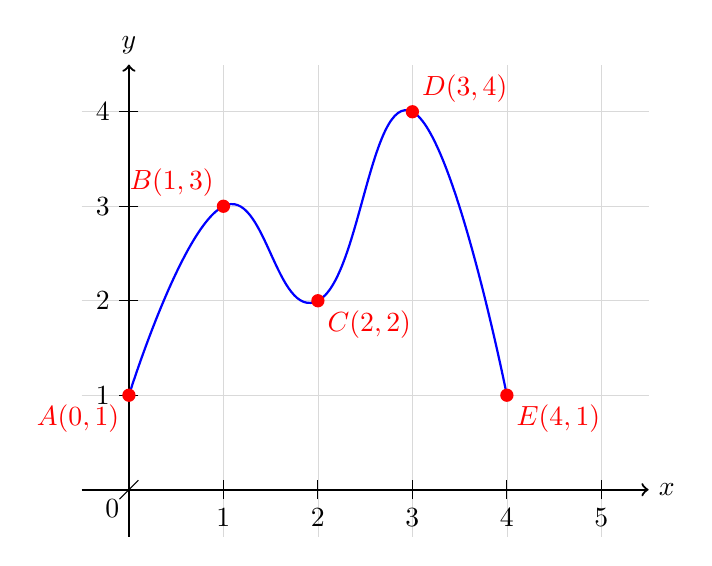
\begin{tikzpicture}[scale=1.2]
    % Grelha
    \draw[step=1cm,gray!30,very thin] (-0.5,-0.5) grid (5.5,4.5);
    
    % Eixos
    \draw[thick,->] (-0.5,0) -- (5.5,0) node[right] {$x$};
    \draw[thick,->] (0,-0.5) -- (0,4.5) node[above] {$y$};
    
    % Marcações nos eixos
    \foreach \x in {1,2,3,4,5}
        \draw (\x,0.1) -- (\x,-0.1) node[below] {$\x$};
    \foreach \y in {1,2,3,4}
        \draw (0.1,\y) -- (-0.1,\y) node[left] {$\y$};
    
    % Origem
    \draw (0.1,0.1) -- (-0.1,-0.1);
    \node[below left] at (0,0) {$0$};
    
    % Função - curva suave passando pelos pontos dados
    \draw[thick, blue] plot[smooth, tension=0.8] coordinates {
        (0,1) (1,3) (2,2) (3,4) (4,1)
    };
    
    % Pontos marcados
    \fill[red] (0,1) circle (2pt) node[below left] {$A(0,1)$};
    \fill[red] (1,3) circle (2pt) node[above left] {$B(1,3)$};
    \fill[red] (2,2) circle (2pt) node[below right] {$C(2,2)$};
    \fill[red] (3,4) circle (2pt) node[above right] {$D(3,4)$};
    \fill[red] (4,1) circle (2pt) node[below right] {$E(4,1)$};
\end{tikzpicture}
\end{center}

\subexercicio{Complete a seguinte tabela de monotonia da função $f$ no intervalo $[0,4]$:}

\begin{center}
\begin{tabular}{|c|c|}
\hline
\textbf{Intervalos} & \textbf{Monotonia} \\
\hline
$]0,1[$ & \underline{\hspace{4cm}} \\
\hline
$]1,2[$ & \underline{\hspace{4cm}} \\
\hline
$]2,3[$ & \underline{\hspace{4cm}} \\
\hline
$]3,4[$ & \underline{\hspace{4cm}} \\
\hline
\end{tabular}
\end{center}

